\documentclass[12pt,letterpaper]{article}
\usepackage{preamble}

\usepackage[utf8]{inputenc}
\usepackage[english]{babel}
\usepackage{listings}
\usepackage{mathtools}
\usepackage{graphicx}
\usepackage{caption}
\usepackage{subcaption}



\newcommand\course{CSE 619}
\newcommand\hwnumber{2}
\newcommand\userID{Max Williams}

\begin{document}

\section{Quiz 2}

\subsection{6.1-4}

The smallest element must be a leaf.

\subsection{6.1-6}

It is not a max heap, because 7 is the child of 6, breaking the max heap rule that a child must be
lesser than its parent.

\begin{figure}[h!]
    \centering
    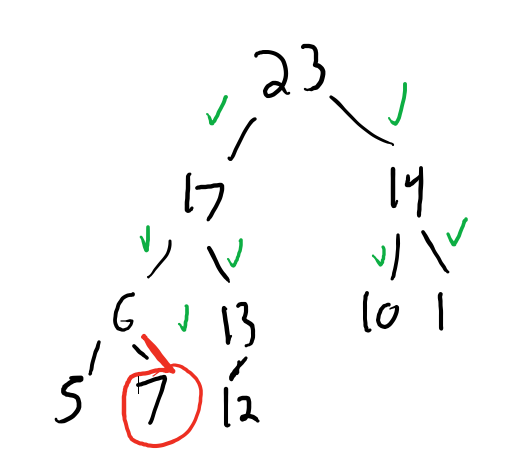
\includegraphics[width=3in]{heap-drawing}
\end{figure}


\subsection{6.4-1}

First, \textsc{max-heapify} is called to make the array into a max heap. Then each step of popping
the top element and \textsc{max-heapify}-ing the heap is shown until only a sorted array is left.


\newcommand{\subfighelper}[1]{
     \begin{subfigure}[b]{0.3\textwidth}
         \centering \includegraphics[width=\textwidth]{#1}
         \caption{}
     \end{subfigure}
     \hfill
 }

\begin{figure}[h!]
     \centering
     \subfighelper{hs1}
     \subfighelper{hs2}
     \subfighelper{hs3}
     \par\bigskip
     \subfighelper{hs4}
     \subfighelper{hs5}
     \subfighelper{hs6}
     \par\bigskip
     \subfighelper{hs7}
     \subfighelper{hs8}
     \subfighelper{hs9}
        \caption{Progression of heap sort. Heapify steps not shown.}
\end{figure}


\subsection{Modular Expontiation}

Do I need to like, make code for this? I guess I'll wait till the asignmetn is up

\end{document}
